\clearpage
\section{Simplified Coherent Receiver}

Student Name: Romil Patel

Starting Date: August 16, 2017

Goal: Develop a simplified structure (low cost) for a coherent receiver, that can be used in coherent PON, inter-data center connections, or metropolitan networks (optical path lengths < 100 km). 

In recent days, homodyne detection has been discussed and investigated a lot due to the advancement in the DSP in the electrical domain. However, a major drawback of homodyne detection is the incoming signal should be separated into inphase and quadrature (I/Q) signals in the optical domain. Therefore, it demands more hardware to accommodate the requirement of the signal separation  in the optical domain. For instance, 4 balanced photodetectors with double hybrid structures and 4-channel ADCs are required.\\
On the other hand, heterodyne receiver simplifies the detection scheme to a great extent with the requirement of having only half of photodetectors and ADCs. A schematic representation of this heterodyne detection system is shown in figure \ref{simplified_coherent_transceiver}.

\begin{figure}[h]
	\centering
	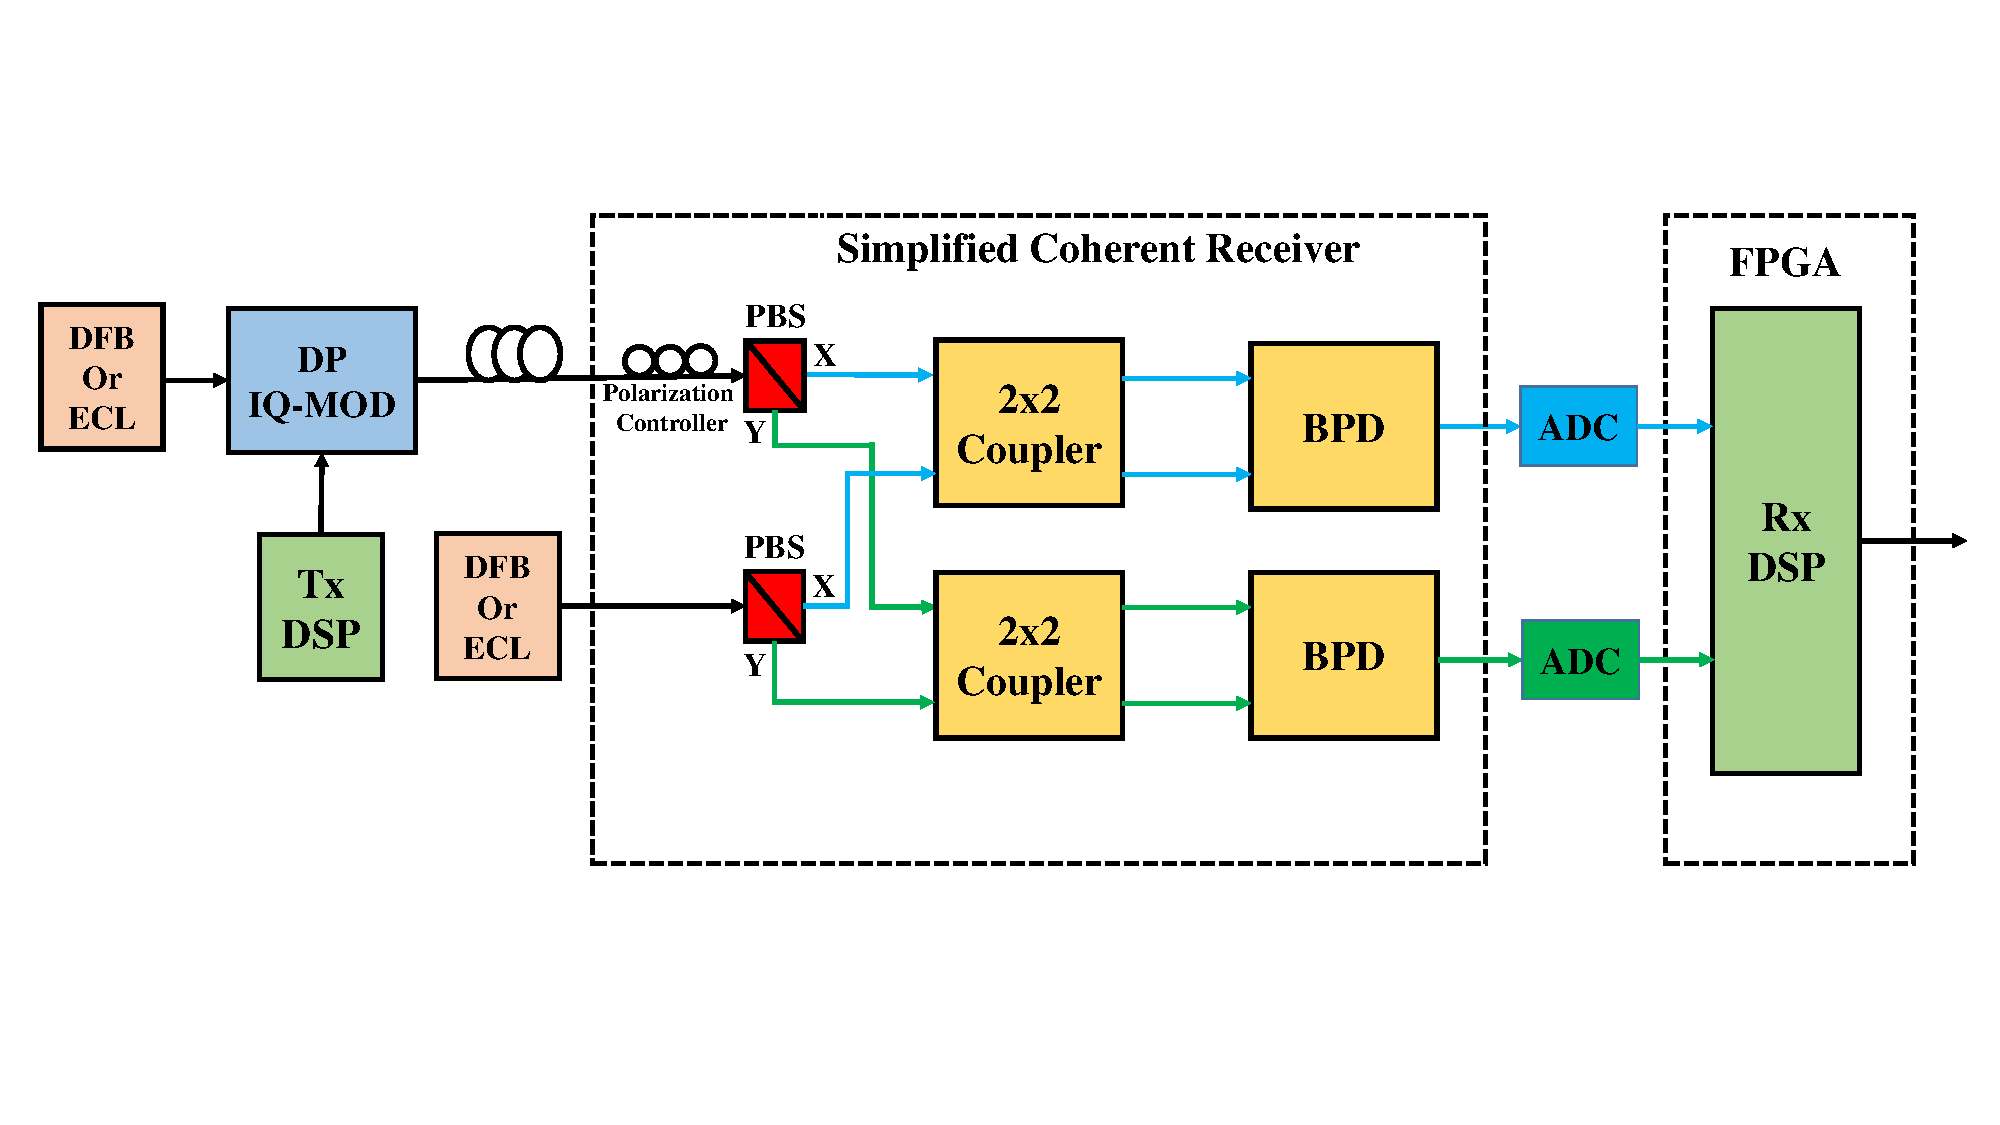
\includegraphics[width=1.0\textwidth, height=7cm]{./sdf/simplified_coherent_receiver/figures/Tx_Rx.pdf}
	\caption{Simplified Coherent Transceiver}\label{simplified_coherent_transceiver}
\end{figure}

\begin{figure}[h]
	\centering
	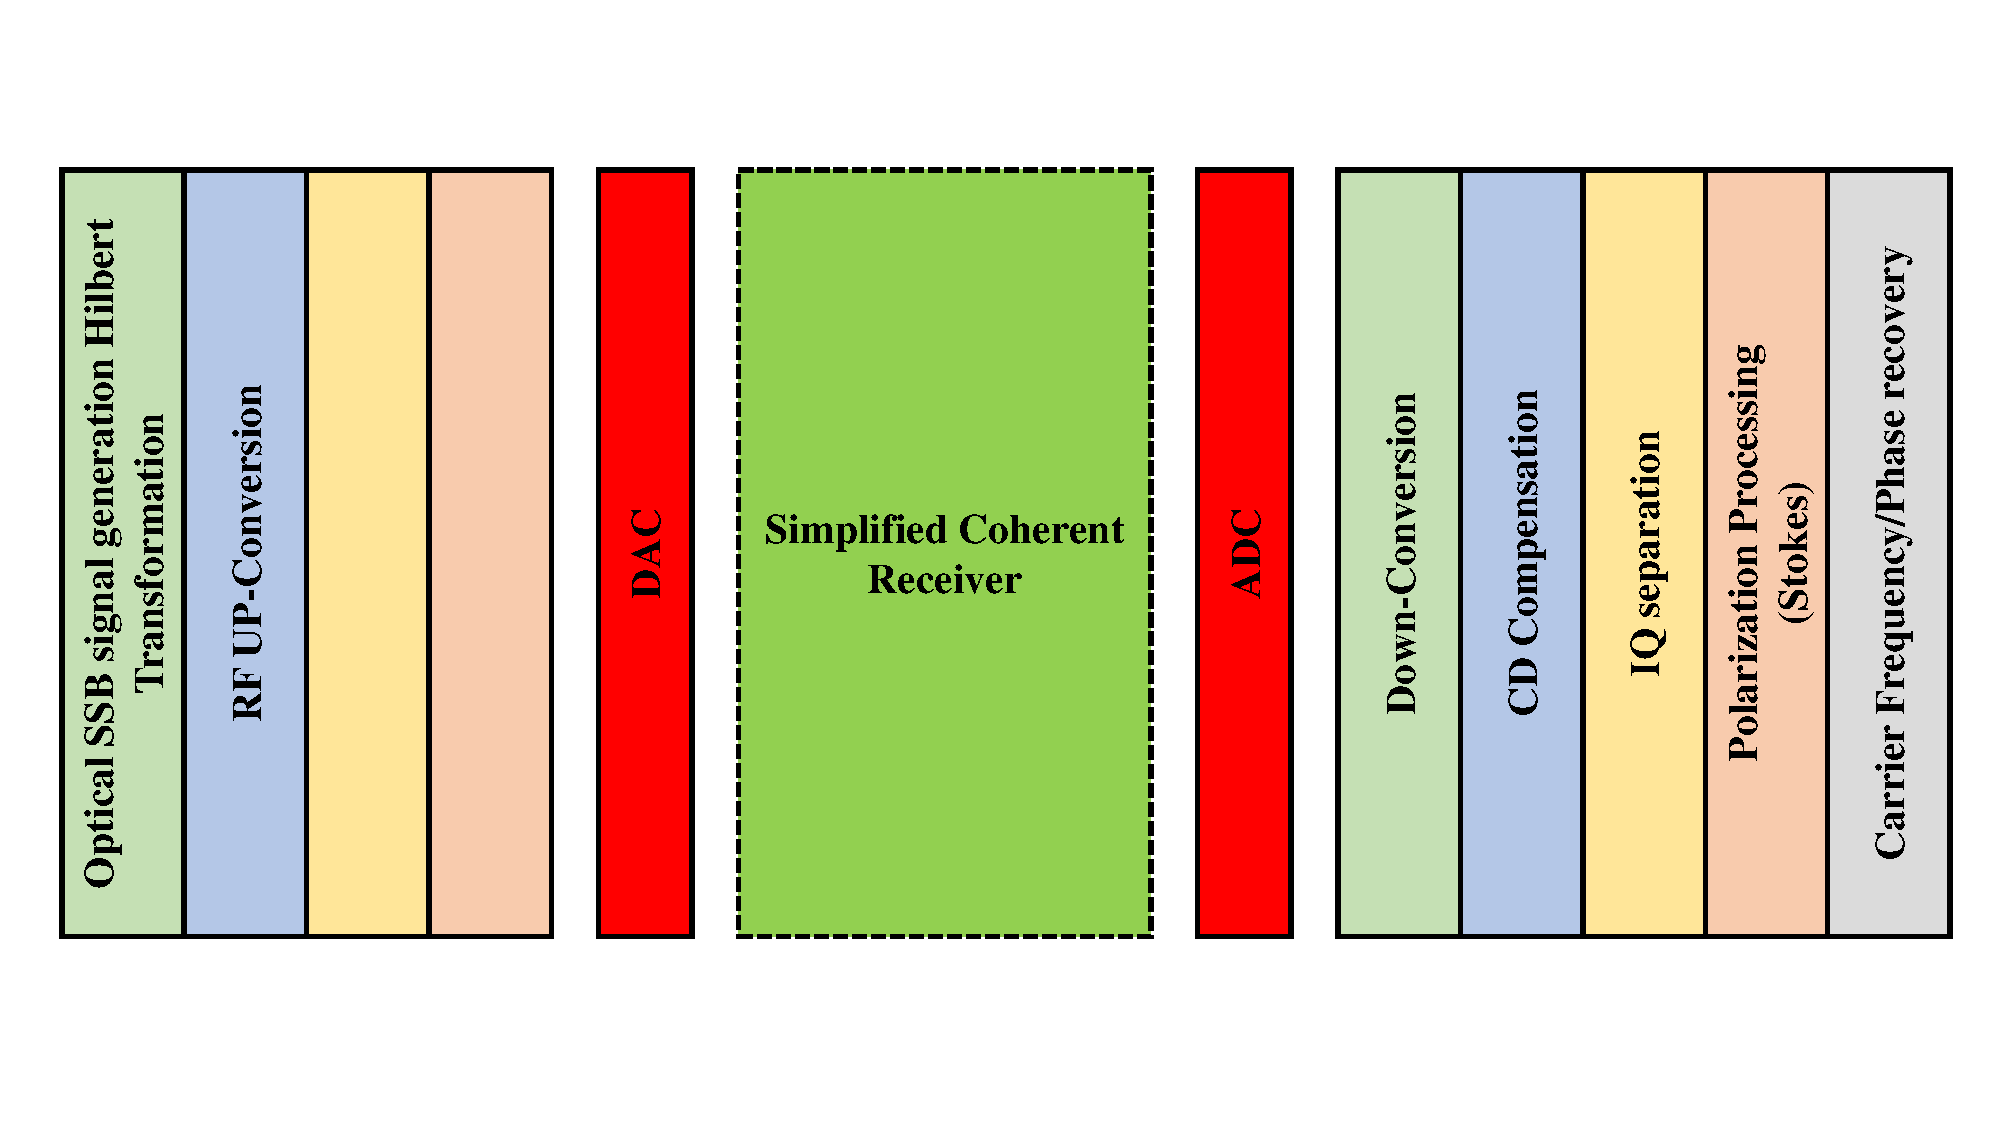
\includegraphics[width=1.0\textwidth, height=7cm]{./sdf/simplified_coherent_receiver/figures/detailed_subsystem.pdf}
	\caption{Tx/Rx DSP main subsystem}\label{DSP_main_subsystem}
\end{figure}

\subsection{Tx side}
Dual polarization(DP) DP-QPSK/DP-16QAM signals (1.25 Gbaud) to be generated at the Tx through an IQ modulator (Figure \ref{DSP_main_subsystem}) driven by DAC mounted in a FPGA. Polarization-division multiplexing is emulated by dividing the signal in two signals using an optical splitter, where a delay of 12 symbols is applied in order to decorrelate the two polarization tributaries and then, both signals are joined orthogonally employing a polarization beam combiner (PBC).

\subsection{Rx side}
At the receiver side, signal is coherently detected using a simplified coherent receiver and a local oscillator. The optical signal is then converted into the electrical domain using two balanced photodetector (BPD), or alternatively four photodetector, and amplified by a transimpedance amplifier (TIA). Following that, the signals are sampled by two 8-bit 2.5 GSa/s ADC and the this digitized signal sent to the FPGA (Virtex-7) where all post-detection DSP implemented in real-time.

